\documentclass[11pt]{article}
\usepackage{fullpage,amsmath,mathtools, algorithm2e, forest}
\usepackage[mathletters]{ucs}
\usepackage{hyperref}
\usepackage[utf8x]{inputenc}
\usepackage{graphicx}
\usepackage{listings}
\usepackage{courier}

\lstset{basicstyle=\footnotesize\ttfamily,breaklines=true}
\lstset{frame=single}

\graphicspath{ {./images/} }
\begin{document}
\title {
    Does misery love company?\\
    Sentiment change over the Twitter social graph\newline\newline
    \large COMP 4601 - Project}
\author{Student Name: Brian Ferch\\
\text{Student Number: 100962115}\\\\ 
Student Name: Jules Kuehn\\
\text{Student Number: 100661464}}
\date{Winter 2019}
\maketitle

% USEFUL EXAMPLE CODE FOR FIGURES AND CODE / TEXT LISTING
% \begin{figure}[h!]
%     \centering
%     \begin{minipage}{0.45\textwidth}
%         \centering
%         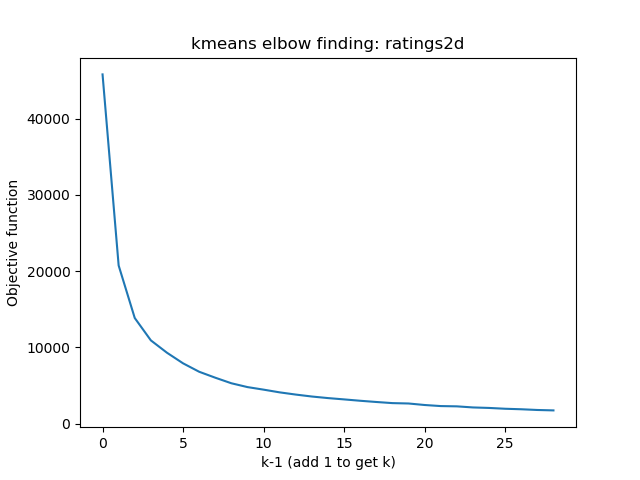
\includegraphics[width=0.9\textwidth]{kmeans_elbow_2d} % first figure itself
%         \caption{Suggests 4 clusters of users}
%     \end{minipage}\hfill
%     \begin{minipage}{0.45\textwidth}
%         \centering
%         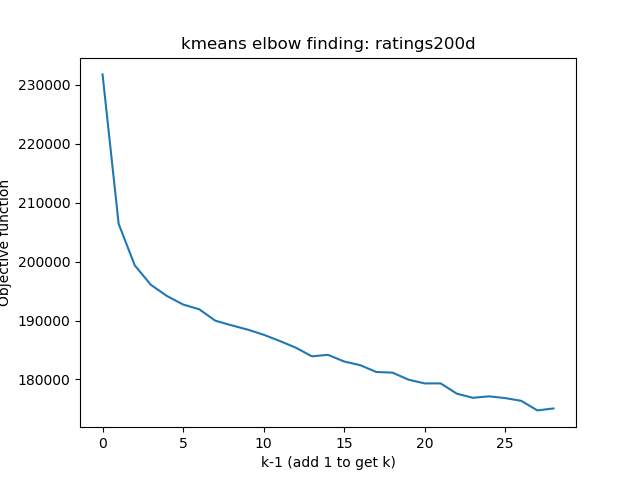
\includegraphics[width=0.9\textwidth]{kmeans_elbow_200d} % second figure itself
%         \caption{Similar results in 200d}
%     \end{minipage}
% \end{figure}

% \lstinputlisting{results/results.txt}

% \begin{figure}[h!]
%     \centering
%      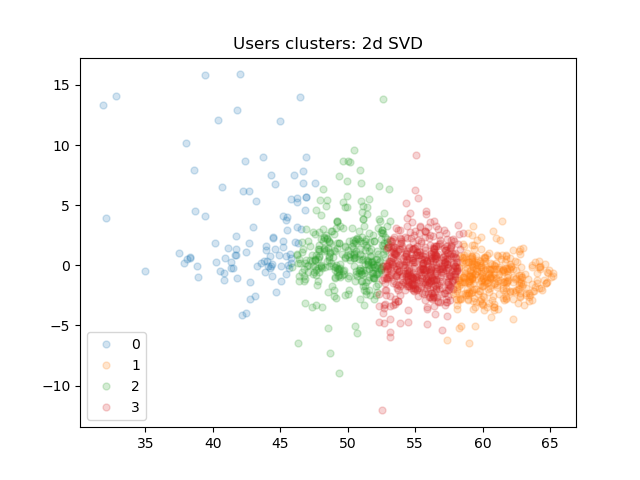
\includegraphics[width=0.5\textwidth]{user_clusters_2d}
%         \caption{Percentage of Recognition Errors}
% \end{figure}


\section{Abstract}

We investigate tweet sentiment over time for 400 socially connected Twitter users by dynamically visualizing changes in tweet sentiment for roughly 400,000 tweets from 2016 to present.\newline

The project scope consists of crawling the social graph, gathering tweets for each user in our graph, translating and analyzing sentiment for each tweet, and visualizing these sentiments over time. Each user is represented as a node, and the color of each node indicates that user’s sentiment at a given time. The graph is displayed using a force-directed layout. From an initial seed node, followers of a user are added along with directed edges for each $(user, follower)$ directed relationship.


\section{Introduction}

A 2015 paper by Tsugawa and Ohsaki[4] found that "negative messages are likely to be reposted more rapidly and frequently than positive and neutral messages". We did not investigate retweets but rather sought to answer whether sentiment spreads more generally between users. This could confirm and expand on the results of that paper, or simply provide some useful insight into the folk wisdom “misery loves company”: that negative sentiment is contagious.\newline

In lieu of any substantial statistical analysis, we visualized the results on an animated graph, allowing for us to explore the data interactively and spot trends.\newline

We will begin with a general overview of the data sources and technologies used and a review of related work. Then we will discuss the specifics of our implementation, and results obtained.


\section{Project overview}

Twitter offers a free rate-limited API which allows us to retrieve the required raw data from queries on a screen name or user id:
\begin{enumerate}
    \item \textbf{userId} : a large integer, ex. 946341920036478976 for our seed user
    \item \textbf{tweets} : most recent $\leq$ 3200 tweets for this user consisting of\newline
    $[(time_1, text_1), (time_2, text_2), \dots]$ 
    \item \textbf{followers} : $[userId_1, userId_2, \dots]$
\end{enumerate}

Many of the gathered users had predominantly non-English tweets. In order to run sentiment analysis with VADER (Valence Aware Dictionary and sEntiment Reasoner)[1] we first had to translate all tweets to English. This was accomplished using Google Cloud Translate, a commercial service.\newline

Based on visual analysis of the data, cleaning was performed programatically. This yielded several datasets usable by the client:
\begin{enumerate}
    \item \textbf{tweets} : all tweets for all users, sorted by time $[(time, userId, sentiment, text), \dots]$
    \item \textbf{users} : information for specific users such as average sentiment, number of tweets, and followers. $\{userId: userInfo, \dots\}$
\end{enumerate}

This data was then displayed as a graph in JavaScript using the d3.js library. Tweet sentiment is then animated over time, as changing color on each node where green is positive sentiment and red is negative. Some smoothing (rolling window averages) is selectively applied to the data to aid in spotting trends at different time granularities.


\section{Methodology}

\subsection{Data acquisition and processing}

Although a historical archive of Twitter data may have been sufficient for our purposes, we opted to acquire some data ourselves via Twitter's API.

\subsubsection{Tools employed}

Cloud services were used heavily in the processing of this data. The data acquisition and processing was all performed on Google Colaboratory's free computing instances, with temporary data stored on a mounted Google Drive for persistence. This allowed us to offload tasks to the cloud which required substantial network activity, processing time, and storage. Processed data was ultimately provided to the visualization client in JSON and CSV formats.\newline

We relied on several Python libraries for specific tasks:
\begin{itemize}
    \item \textbf{Tweepy} for calling the Twitter API
    \item \textbf{nxGraph} for creating a user graph and performing page rank
    \item \textbf{VADER} for analyzing tweet sentiment
    \item \textbf{matplotlib} for inspecting the data while cleaning
    \item \textbf{numpy} for numerical processing and matrix manipulation
\end{itemize}

Most of the above are standard tools for these uses in Python. For the crucial task of sentiment analysis, we chose VADER becaus unlike mainstream libraries such as CoreNLP, VADER is specially tuned to analyse social media text. It is able to recognize emoticons such as :) and Unicode emoji, and also takes capitalization and punctionation such as ALLCAPS!!! into account for sentiment analysis.\newline

Twitter's free API was sufficient for extracting 400 users and up to 3200 tweets each. (Rate-limiting made it impossible to achieve a larger crawl in the time-frame we had.) Google Translate's free API was however insufficient due to both rate limiting and issues decoding Unicode emoji. Google's commercial Cloud Translate service was up to the task, after rate limits were manually increased to 10 million characters per 100 minutes.\newline

\subsubsection{Methodology}

\textbf{Seed user:} First, we identified a seed node. After some experimentation with using popular celebrity accounts as seed nodes, quick inspection of the resultant graph showed that it was too broad and not deep enough for the desired visualization. We found that using a normal, less popular user resulted in a graph better conforming to our intent (See Figure 5). This user was selected by browsing followers of the City of Ottawa account. Our seed user is local to Ottawa, and has only 2 tweets and 13 followers. (In retrospect, a user with more moderate activity (hundreds of tweets, dozens of followers) would have likely produced better results.)\newline

\textbf{Building a graph:} Crawling the user graph had already been implemented simply in Python by Yuya Takashina's twicrawler[3]. We used this as base code, making modifications to crawl 'forward' through a potential chain of influence by adding a seed user's followers to a priority queue. The priority was determined by the PageRank score of that user's node in the partially acquired social graph. The aim was to process more popular users first, as we assumed these users would be of higher quality and influence.

From this graph of user nodes, we removed all but the 400 highest page-ranked nodes.\newline

\textbf{Getting tweets:} Then, for each of the 400 user nodes, we retrieved the last 3200 tweets from each user using Tweepy based on an existing script[5]. This retrieved the tweets in batches of 200. We frequently ran into rate-limiting and had to run the script at intervals on appropriately sized mini-batches of users.\newline

We then roughly followed the tutorial "(Almost) Real-Time Twitter Sentiment Analysis with Tweep \& Vader"[2]. Tweets were cleaned of links, retweet handles, user handles, and special characters (leaving emoji). The tweets were sent in batches to Cloud Translate, and the translated text was analysed for sentiment with VADER, yielding positive, neutral, negative, and compound sentiment scores for each tweet. We wanted a single real number for our sentiment visualization, so we stored only the compound sentiment score along with each tweet.\newline

\textbf{Inspecting and processing data:} We now have all $tweets$ for all users, sorted by time and scored with compount sentiment $[(time, userId, sentiment, text), \dots]$. We gather together some useful information on the users from the graph and tweets into $users$. This includes the followers of that user (nodes connected through out-edges on the graph), and the average sentiment scores. A second average is made of non-zero sentiments.\newline
The raw sentiment values of all tweets over time is shown in Figure 1. Manual inspection of zero-sentiment tweets showed that many were of low quality (tweets which were simply URLs, stripped characters, or poorly translated). Therefore, the zero-sentiment tweets were removed. The non-zero average for each user was then subtracted from each of that user's sentiments $s$:

\[
    s_{new} = s_{raw} - avg(s\in tweets_{user}, s \neq 0)
\]

As our visualization is time based, we want to make sure we have sufficient tweet density for a useful visualization at a given time. Inspecting the timestamps of the tweets showed that less than 10\% of gathered tweets occured between 2009 and 2016 (see Figure 6). The processed \textbf{tweets} list now consists only of non-neutral tweets from January 1, 2016 to the crawl date April 13, 2019, with sentiment scores normalized by user average. We are left with 61.6\% of the total tweets gathered, but de-noised and with sentiment value somewhat exagerrated, making it easier to visualize change in sentiment.

\begin{figure}[h!]
    \centering
    \begin{minipage}{0.45\textwidth}
        \centering
        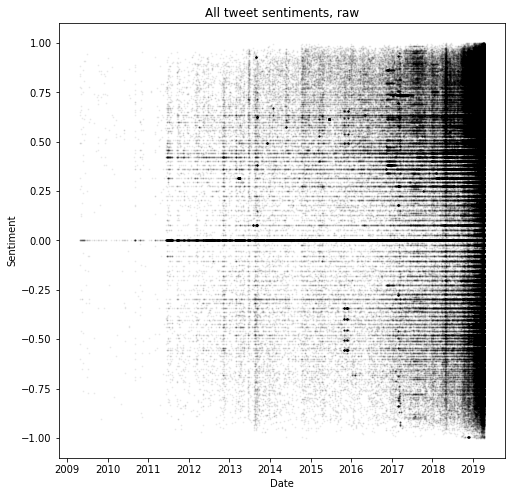
\includegraphics[width=0.9\textwidth]{raw_sentiments} % first figure itself
        \caption{Raw sentiments}
    \end{minipage}\hfill
    \begin{minipage}{0.45\textwidth}
        \centering
        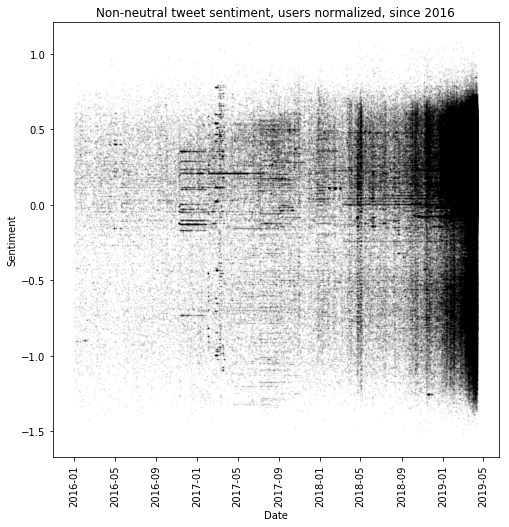
\includegraphics[width=0.9\textwidth]{nnz_since_2016} % second figure itself
        \caption{Processed sentiments}
    \end{minipage}
\end{figure}

The time granularity of this data was very fine (by second) at this point, making it unsuitable for animation over several years. To compensate for this, and to smooth sentiment values for more useful visualization, we employed several rolling window averages:\newline
\begin{itemize}
    \item 3 day window, 1 day step (length: 1199)
    \item 1 week window, 3 day step (length: 400)
    \item 2 week window, 3 day step (length: 400)
    \item 4 week window, 3 day step (length: 400)
\end{itemize}

Users who did not make any tweets in that time window are not given an average sentiment for that window.\newline

To better understand the data, we plotted the averages for each of these windows. We can see that increasing the window size shows less granular trends over months while the smallest window size shows more granular trends over weeks and even days (see Figures 3 and 4).

\begin{figure}[h!]
    \centering
     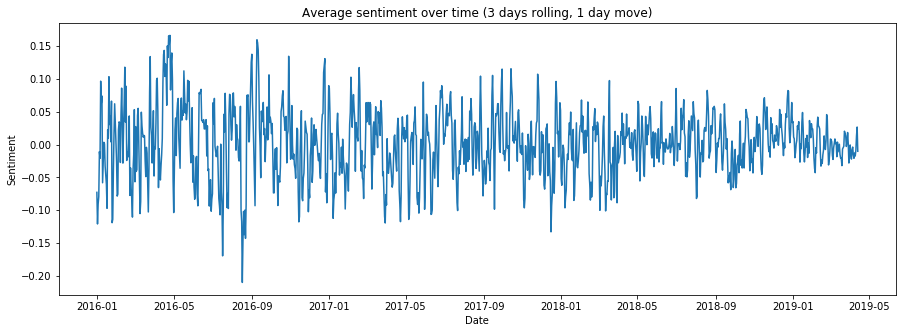
\includegraphics[width=0.8\textwidth]{avg_sentiment_over_time_big__3day}
        \caption{Average tweet sentiment for all users, 3 day rolling window}
\end{figure}

\begin{figure}[h!]
    \centering
     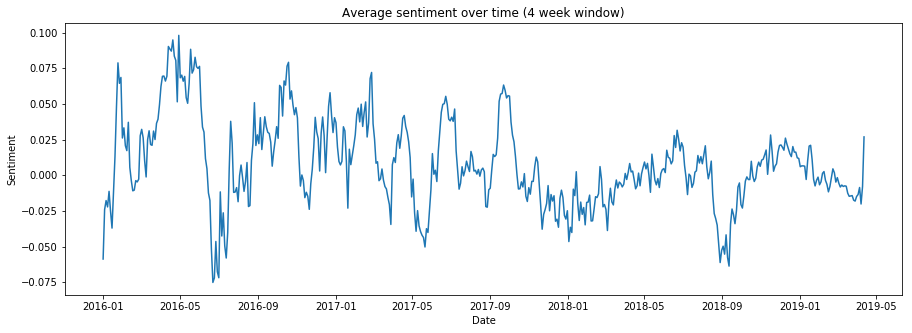
\includegraphics[width=0.8\textwidth]{avg_sentiment_over_time_big_4week}
        \caption{Average tweet sentiment for all users, 4 week rolling window}
\end{figure}

\subsection{Visualization}
Add this \dots\newline

Include figures of some sentiment bouncing around a local community over adjacent time window, confirming 2nd paragraph of Discussion below. I can do figures syntax

\subsubsection{Tools employed}
node, d3.js

\subsubsection{Methodology}
force directed graph\newline

how data was processed from what i provided

d3.js is a powerful data visualization library that specializes in creating complex and dynamic data representations.
For our visualization we used a force directed graph for it's ability to display a large amount of connected data that is still
visually digestible and aesthetically pleasing.

Even with a powerful library like d3.js, it can still be very difficult to construct a graph that animates over time with the data.
We started with some base code that gave us the basic style and format of the graph [https://observablehq.com/@d3/force-directed-graph].

The initial static construction of the graph was fairly trivial. The sentiment value of each node was interpolated as a color, with -1
being bright red, and 1 being bright green. True neutral values were given gray.

Connections in d3 graphs are constructed as a list of sources and targets. For our sources, we used the followers, our targets 
were the people being followed. A client side preprocessing step was needed to build this list.

To add animation to the graph, we loop through the rolling average windows and interpolate the color between subsequent sentiments
in subsequent windows. Each window takes a certain length of time to animate between which can be adjusted with the "Speed" input.

We also added the ability to choose and visualize a specific date, and visualize where along the entire canonical time period of the data
you were currently with the addition of the range slider. Different windows can be scrubbed to with the slider, and the corresponding
sentiment colors are rendered to the nodes.


\section{Discussion}
The windowed averages shown in Figures X-X demonstrate that sentiment trends have definitely been captured in the data. We can infer that certain historical events caused certain shifts in overall sentiment by looking at the dates, and also see different users react to those events in terms of change in their sentiment.\newline

Close visual inspection of clusters over time indicates that there is some relationship between adjacent users' average sentiments (see Figures X-X). Specifically, changes in the sentiment of adjacent users often occurs sequentially over a few windows. Since there are bidirectional relationships present, it is difficult to make a strong judgement on our initial hypothesis: that (negative) sentiment spreads between socially adjacent users over time, that is, directional relationships.\newline

We can see that certain sentiments appear in certain socially adjacent groups around the same time, independently of the overall average sentiment. This implies that you are more likely to share sentiment over a window of time with those in your close social community than with random other users, and that the community, even sampled from a single seed, is heterogenous while still showing clear overall trends.\newline

As previously mentioned, Twitter rate limits and limitations on our own time were causes of difficulty, along with text encoding issues in translation. But the various APIs and cloud services employed delivered a usable data set for a viable proof-of-concept implementation, and a glimpse at what results might appear with a more comprehensive approach to this problem.


\section{Future work}
The work could be improved with better data (more seeds), in the same format. Some other useful information to graph might be the language of the users, such that communities of different language, and the links between them, can be visualized. Translated tweets should also be stored, rather than discarded after scoring sentiment. Scored tweets from a user over a particular time window could be displayed when hovering on that node. User screen names and profile images could also appear in this card.\newline

With the data already gathered, there is more that could be displayed. Particularly negative sentiment tweets could be identified around a sudden drop in average sentiment in order to identify the likely cause of the negative sentiment. Community identification could be inferred from tweet text using document vectors etc., by social proximity, or by sentiment over time. For the latter method, we think of the users as 'rating' a period in time (the rolling window). Then, their sentiments can be represented as a ratings matrix and SVD dimensionality reduction, clustering etc. could be performed.\newline

Community improvements to the visualization component are possible on GitHub Since the data processing scripts are both available and runnable in Google Colaboratory, different datasets can be gathered and then visualized.


\section{Conclusion}
Summarize the content of the report with a focus on the goal, analysis, and resulting value. Recap relevant points from the discussion, but do not restate it. Finally, you can choose to touch on future works as you close out the paper.\newline

We began with a goal of confirming whether indeed “misery loves company” on Twitter, and specifically if sentiment shows a directed movement across the Twitter social graph.\newline

We visualized tweet sentiment over time for 400 users crawled from a single seed user. We binned 396,937 tweets from 2016-01-01 to 2019-04-13 into rolling averages over time windows, at different granularity of window size and step. By visual inspection, we found certain patterns which both addressed our goal for the analysis, and provided additional insights into communities on Twitter.\newline

Related to our goal, we found that change in the sentiment of adjacent users does tend to occur at similar times, and in sequence rather than in parallel. However, we could not confirm a directional relationship within the graph, as would be required to show that negative sentiment is spreading directionally. In reality, the sources of change in user sentiment are probably too complex to be modeled in this kind of causal relationship, and it would be surprising to see a strong demonstration of this in a random sample of the social graph.\newline

Additionally, we found that certain socially-close communities of sentiment-over-time emerge, distinct from overall sentiment. Overall sentiment also showed a distinct trend, and based on the dates we can infer relationships to world events. Future work could better explore sources of negative sentiment.\newline

We found that visualizing sentiment over the Twitter user graph is illuminating and compelling. By publishing an example of crawling and processing code on Google Colaboratory, others can gather larger datasets, perhaps ones focusing on specific communities. By publishing our visualization code on GitHub, we provide a full solution for visualizing sentiment on parts of the social graph which are of interest to the user with minimal fuss.

\appendix
\section{\\Appendix}

\begin{figure}[h!]
    \centering
     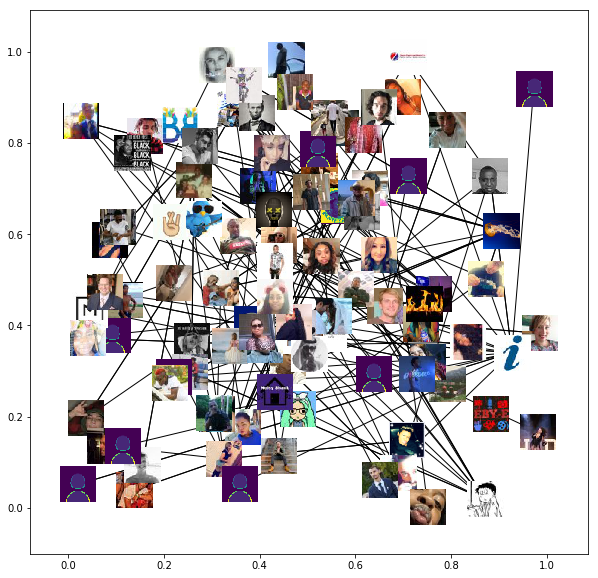
\includegraphics[width=0.5\textwidth]{nxgraph_unpopular_seed}
        \caption{Highest PageRanked users from unpopular seed user}
\end{figure}

\begin{figure}[h!]
    \centering
     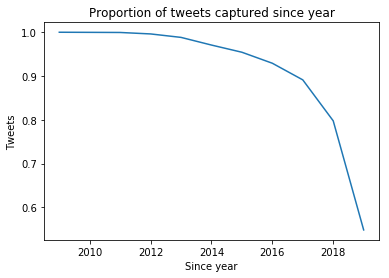
\includegraphics[width=0.5\textwidth]{tweets_since_year}
        \caption{Percentage of total tweets captured by starting year}
\end{figure}

\section{\\References}

[1] Hutto, C.J., and Eric Gilbert. “VADER: A Parsimonious Rule-Based Model for Sentiment Analysis of Social Media Text,” 2015.\newline

[2] Rovai, Marcelo. “(Almost) Real-Time Twitter Sentiment Analysis with Tweep \& Vader.” Towards Data Science, December 27, 2018. https://towardsdatascience.com/almost-real-time-twitter-sentiment-analysis-with-tweep-vader-f88ed5b93b1c.\newline

[3] Takashina, Yuya. Crawling the Social Graph on Twitter. Jupyter Notebook, 2017.\newline
https://github.com/ytakashina/twicrawler.\newline

[4] Tsugawa, Sho, and Hiroyuki Ohsaki. “Negative Messages Spread Rapidly and Widely on Social Media,” 151–60, 2015. https://doi.org/10.1145/2817946.2817962.\newline

[5] Zmick, David. tweet\_dumper.py. Python, 2019. https://github.com/dpzmick/one-liners.


\end{document}